\documentclass[aspectratio=169,t]{beamer}

% Clean academic look: white background, no decorations, generous whitespace.
\usetheme{default}
\setbeamertemplate{navigation symbols}{}
\setbeamercolor{background canvas}{bg=white}
\setbeamercolor{normal text}{fg=black!88}
\setbeamercolor{frametitle}{fg=black}
\setbeamerfont{frametitle}{size=\Large, series=\bfseries}
\setbeamertemplate{frametitle}{%
  \vspace{0.7em}\hspace{0.5em}\insertframetitle\par%
  \vspace{0.2em}\hspace{0.6em}{\small\color{black!55}\insertframesubtitle}\par}
\setbeamertemplate{footline}{%
  \hfill\scriptsize\color{black!35}\insertframenumber\;/\;\inserttotalframenumber\hspace{1em}\vspace{0.5em}}
\setbeamertemplate{itemize item}{\textbullet}
\setbeamertemplate{itemize subitem}{\textendash}

\usepackage{booktabs}
\usepackage{amsmath, amssymb}
\usepackage{xcolor}
\usepackage{graphicx}
\usepackage{tabularx}
\usepackage{array}

% Compact tables, gentle row spacing
\renewcommand{\arraystretch}{1.10}

% Where ggsave outputs live (relative to the .tex compile dir)
\graphicspath{{./}{../figs/}{../figs/longitudinal/}{../figs/io/}{../figs/proc/}{../figs/schematic/}}

% Convenience commands
\newcommand{\pia}{\pi_{\alpha}}
\newcommand{\sigxi}{\sigma_{\xi}}
\newcommand{\siga}{\sigma_{\alpha}}
\newcommand{\sigr}{\sigma_{r}}
\newcommand{\sigz}{\sigma_{\zeta}}
\newcommand{\siglam}{\sigma_{\lambda}}

% Accent: brand-red used for the "kid" / acceleration thread
\definecolor{accent}{RGB}{195,30,55}
\definecolor{cool}{RGB}{31,120,180}

\title{\bfseries Variability and acceleration in the\\growth of children's early vocabulary}
\subtitle{}
\author{Michael C.\ Frank}
\institute{\small Stanford University}
\date{2026}

\begin{document}

% =====================================================================
\begin{frame}[plain]
\titlepage
\end{frame}

% =====================================================================
\begin{frame}{Vocabulary growth: rapid, variable, consequential}

\begin{columns}[T, onlytextwidth]
\column{0.55\textwidth}
\textbf{Theoretical:} Growth mechanisms are diagnostic of how
children's learning works --- and how it changes with development.

\vspace{1em}
\textbf{Practical:} Variation in vocabulary growth is a key precursor
of academic outcomes.

\vspace{1em}
\textbf{Methodological:} Vocabulary count has a property nearly no
other psychological metric has --- a \emph{true zero}. Children at
birth know zero words. Absolute variability in word counts is
interpretable, not just z-scores.

\column{0.45\textwidth}
\centering
\includegraphics[width=\linewidth]{precursor_trajectories.png}

\vspace{0.3em}
\scriptsize\color{black!55}\textit{Per-admin theta on Wordbank
longitudinal sample. Each grey line = one child.}
\end{columns}

\end{frame}

% =====================================================================
\begin{frame}{Two signatures of vocabulary growth}{What any theory of word learning has to predict}

\begin{columns}[T, onlytextwidth]

\column{0.5\textwidth}
\centering
\textbf{\large\color{accent} Variability}\\[0.4em]
\small
Children fan out, not converge. \\[0.4em]
Within-age SD of ability \emph{grows} with age. \\[0.6em]

\vspace{0.2em}
\includegraphics[width=0.95\linewidth]{precursor_variation.png}

\column{0.5\textwidth}
\centering
\textbf{\large\color{accent} Acceleration}\\[0.4em]
\small
Vocabulary grows super-linearly in tokens. \\[0.4em]
Population scaling exponent $\kappa_{\text{pop}} \gg 1$. \\[0.6em]

\vspace{0.2em}
\includegraphics[width=0.95\linewidth]{m_best_spaghetti.png}

\end{columns}

\vspace{0.4em}
\centering
\small\color{black!55}\textit{Both signatures show up in nearly every
language Wordbank covers (next slide).}

\end{frame}

% =====================================================================
\begin{frame}{Cross-language replication}{Variability and growth-with-age across Wordbank languages}

\centering
\includegraphics[width=0.78\linewidth]{precursor_crosslang_overlay.png}

\vspace{0.4em}
\small
\textbf{Variability is universal} --- and grows with age in every sampled language.
Each grey line is one language's within-age SD of $\theta_{\text{admin}}$;
red is the cross-language mean.

\end{frame}

% =====================================================================
\begin{frame}{The structural null: pure accumulator}

\begin{columns}[T, onlytextwidth]
\column{0.55\textwidth}
\small
\textbf{Pure accumulator.}
Each child accumulates word-evidence at per-child input rate $r_i$;
word $j$ is acquired when difficulty $\delta_j$ is crossed.

\vspace{0.4em}
\textbf{Scaling exponent $\kappa_i$:} ability scales as (tokens)$^{\kappa_i}$.

\begin{itemize}\setlength\itemsep{0.15em}
\item $\kappa_i = 1$ for every child: pure unit accumulator.
\item Between-child variance comes only from $\sigma_r$ (input rate).
\item No per-child slope variation.
\end{itemize}

\vspace{0.4em}
\textbf{Two estimands diagnose deviation:}
$\boldsymbol{\sigma_\alpha}$ (efficiency variation) and the $\boldsymbol{\kappa_i}$
posterior (\emph{is $\kappa$ above 1, and does it vary?}).

\column{0.45\textwidth}
\centering
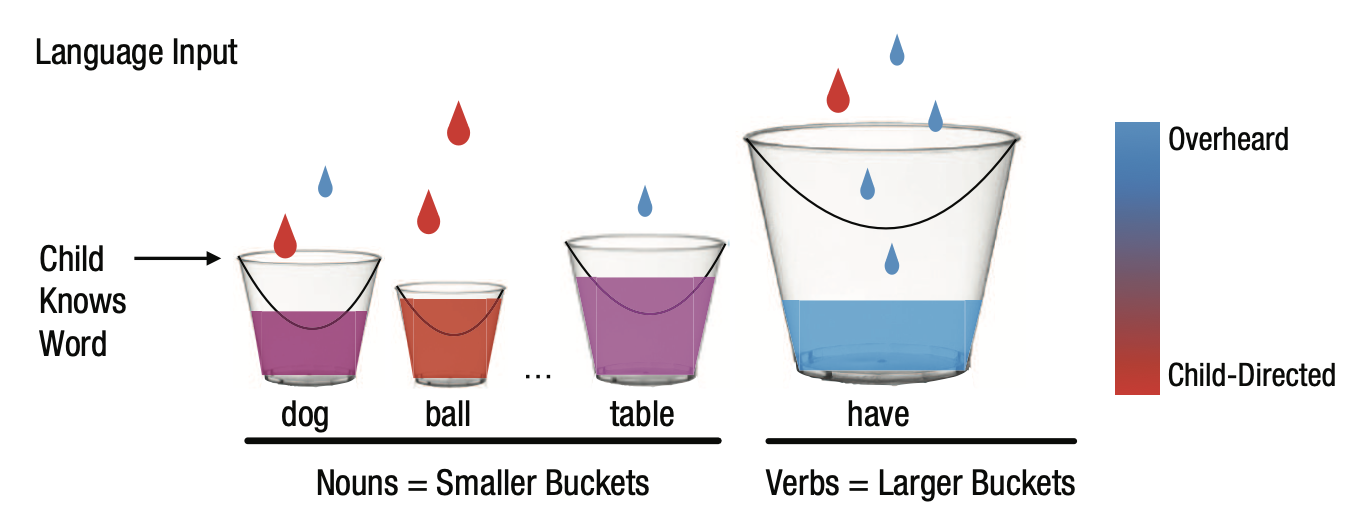
\includegraphics[width=0.92\linewidth]{kachergis_buckets.png}

\vspace{0.3em}
\scriptsize\color{black!55}\textit{Bucket-fill metaphor: each child
hears tokens at rate $r_i \cdot p_j$; word $j$ is acquired when its
bucket fills past difficulty $\delta_j$ (Kachergis et al.\ 2021).}
\end{columns}

\end{frame}

% =====================================================================
\begin{frame}{Where prior accumulator models sit}{None has both $\sigma_\alpha$ and $\sigma_\kappa$ free}

\centering
\scriptsize
\renewcommand{\arraystretch}{1.30}
\begin{tabular}{@{}lp{2.0cm}p{2.0cm}p{4.5cm}@{}}
\toprule
\textbf{Model} & \textbf{per-child $\sigma_\alpha$} & \textbf{per-child $\sigma_\kappa$} & \textbf{$\kappa_{\text{pop}} > 1$ via} \\
\midrule
McMurray (2007) pure accumulator        & --        & --        & only via $g'(\tau)$ \\
Mitchell \& McMurray (2009) + leverage  & --        & --        & shifts but cannot create \\
Hidaka (2013) closed-form AoA           & --        & --        & rate-change exponent $D$ \\
Mollica \& Piantadosi (2017) Gamma      & --        & --        & embedded in per-word $\lambda_w$ \\
Kachergis et al.\ (2021) 1-PL Rasch     & $\theta_i$ free   & --   & linear age covariate \\
\midrule
\textbf{M\_best (this work)}            & \textbf{free}     & \textbf{free}     & \textbf{free} \\
\bottomrule
\end{tabular}

\vspace{1.0em}
\small
\textbf{Common gap.} No prior accumulator model has both $\sigma_\alpha$
\emph{and} $\sigma_\kappa$ free. Most have neither. The two signatures
we measure --- variability and acceleration --- are precisely what
these models cannot produce.

\end{frame}

% =====================================================================
\begin{frame}{The model: a progressive build}{Rasch IRT + accumulator dynamics, in three steps}

\footnotesize
Kid $i$, word $j$: \;\; $P(\text{produces}_{ij}) = \sigma(\eta_{ij})$, with
$\eta_{ij} = \theta_i - \delta_j$ \;\; (ability $-$ difficulty).

\vspace{0.3em}

\textbf{Step 1 -- Pure accumulator.}\;
$\theta_i = \log r_i + \log t \;\;\Longleftrightarrow\;\; \exp(\theta_i) = r_i \cdot t$

\emph{Ability = rate $\times$ time. Variation between kids comes only from $r_i$.}

\vspace{0.3em}

\textbf{Step 2 -- + per-child efficiency $\alpha_i$.}\;
$\theta_i = \log r_i + \log \alpha_i + \log t \;\;\Longleftrightarrow\;\; \exp(\theta_i) = \alpha_i \cdot r_i \cdot t$

\emph{Each child has a multiplicative efficiency over and above input rate.}

\vspace{0.3em}

\textbf{Step 3 -- + per-child scaling exponent $\kappa_i$.}\;
$\theta_i = \log r_i + \log \alpha_i + \kappa_i \log t \;\;\Longleftrightarrow\;\; \exp(\theta_i) = \alpha_i \cdot r_i \cdot t^{\kappa_i}$

\emph{Children also differ in how steeply ability scales with cumulative input.}

\vspace{0.6em}

\textbf{Two diagnostic questions:}\quad
$\pi_\alpha = \dfrac{\sigma_\alpha^2}{\sigma_\alpha^2 + \sigma_r^2} > 0.5\,$? \;\;
(efficiency-share of variance)
\quad
$\kappa_i > 1\,$? \;\;
(super-linear scaling)

\end{frame}

% =====================================================================
\begin{frame}{M\_best fit: per-child trajectory fan}{120 kids drawn from posterior of \texttt{long\_no\_freq\_slopes}}

\centering
\includegraphics[width=0.96\linewidth]{m_best_spaghetti.png}

\vspace{0.4em}
\small
\textbf{Left:} ability $\theta_{it}-\mu_r$ vs.\ $\log_{age}$, slope = $\kappa_i$, mean $\approx 10.4$.\quad
\textbf{Right:} same kids, vocabulary on linear age. Median tracks Wordbank empirical.

\end{frame}

% =====================================================================
\begin{frame}{M\_best parameters}{Variability and acceleration both bounded firmly above zero}

\centering
\small
\renewcommand{\arraystretch}{1.20}
\begin{tabular}{@{}llp{8cm}@{}}
\toprule
\textbf{Parameter} & \textbf{Posterior} & \textbf{What it does} \\
\midrule
$\sigma_\alpha$   & 1.71 \,[1.55, 1.91]   & Between-child efficiency variation. \\
$\boldsymbol{\pi_\alpha}$ & \textbf{0.91 \,[0.89, 0.93]} & \textbf{Share of intercept variance from efficiency, not input.} \\
$\boldsymbol{\kappa_{\text{pop}}}$ & \textbf{10.35 \,[10.21, 10.51]} & \textbf{Population scaling exponent: ability scales as (tokens)$^{\kappa}$.} \\
$\boldsymbol{\sigma_\kappa}$ & \textbf{3.47 \,[3.14, 3.84]} & \textbf{Between-child variation in scaling exponent.} \\
$\rho(\xi,\kappa)$ & $+0.35$ \,$[+0.22, +0.47]$ & Higher-baseline kids have steeper growth. \\
\bottomrule
\end{tabular}

\vspace{0.8em}

\begin{columns}[T, onlytextwidth]
\column{0.32\textwidth}
\centering\textbf{\color{accent}Variability}\\[0.2em]
\small
$\pi_\alpha = 0.91$: efficiency variance dominates input variance.

\column{0.32\textwidth}
\centering\textbf{\color{accent}Acceleration}\\[0.2em]
\small
$\kappa_{\text{pop}} \approx 10.4 \gg 1$: scaling is wildly super-linear, far from the unit accumulator.

\column{0.36\textwidth}
\centering\textbf{\color{accent}Variation in scaling}\\[0.2em]
\small
$\sigma_\kappa > \sigma_\alpha$: kids vary more in scaling exponent than in baseline.

\end{columns}

\end{frame}

% =====================================================================
\begin{frame}{Where between-child variance comes from, by age}{$\pi_\alpha$ is exact at $a_0$ and qualified elsewhere}

\centering
\includegraphics[width=0.85\linewidth]{m_best_variance_decomp.png}

\vspace{0.4em}
\small
\textbf{At the pivot age (19 mo):} only input + efficiency contribute $\Rightarrow \pi_\alpha = \sigma_\alpha^2/(\sigma_\alpha^2 + \sigma_r^2)$ exact.\quad
\textbf{Off-pivot:} scaling variance $\sigma_\kappa^2 \cdot \log_{age}^2$ dominates by 30 mo.

\end{frame}

% =====================================================================
\begin{frame}{Cross-sample variability: $\pi_\alpha$ replicates}{Five samples, two languages, three input-observation channels}

\centering
\small
\renewcommand{\arraystretch}{1.20}
\begin{tabular}{@{}lrcc@{}}
\toprule
\textbf{Sample} & \textbf{N} & $\boldsymbol{\sigma_\alpha}$ & $\boldsymbol{\pi_\alpha}$ \\
\midrule
English Wordbank longitudinal           & 200 & 1.83 \,[1.65, 2.04]     & 0.91 \,[0.90, 0.93] \\
Norwegian Wordbank longitudinal         & 200 & 2.10 \,[1.90, 2.35]     & 0.94 \,[0.93, 0.95] \\
BabyView (head-mounted video)           &  20 & 1.13 \,[0.86, 1.61]     & 0.84 \,[0.68, 0.93] \\
SEEDLingS (LENA + comp correction)      &  44 & 1.39 \,[1.13, 1.74]     & 0.94 \,[0.89, 0.97] \\
Peekbank-Stanford (LWL processing)      &  62 & 1.64 \,[1.34, 2.03]     & 0.90 \,[0.86, 0.94] \\
\bottomrule
\end{tabular}

\vspace{1em}

\textbf{Headline.} $\pi_\alpha \in [0.84, 0.94]$ across every well-conditioned sample. \\
\textbf{Input rate quantity explains $<\!10\%$ of between-child intercept variance.}

\vspace{0.6em}
\small\color{black!55}\textit{Cross-channel replication: directly observed input (BabyView, SEEDLingS), inferred input (Wordbank), processing-coupled (Peekbank). SEEDLingS extreme corrected for parent-report noise via comprehension channel.}

\end{frame}

% =====================================================================
\begin{frame}{Cross-language acceleration: where it lives, not whether it does}

\centering
\small
\renewcommand{\arraystretch}{1.20}
\begin{tabular}{@{}lcccc@{}}
\toprule
\textbf{Sample} & \textbf{admins/kid} & $\boldsymbol{\kappa_{\text{pop}}}$ & $\boldsymbol{\sigma_\kappa}$ & \textbf{kid range ($\kappa_{\text{pop}} \pm 2\sigma_\kappa$)} \\
\midrule
English   & median 3 & 10.4 \,[10.2, 10.5] & 3.5 \,[3.1, 3.8] & $\sim$3 to 17 \\
Norwegian & median 8 & 12.4 \,[12.3, 12.6] & 3.7 \,[3.4, 4.2] & $\sim$5 to 20 \\
\bottomrule
\end{tabular}

\vspace{0.8em}

\begin{columns}[T, onlytextwidth]
\column{0.55\textwidth}
\textbf{Population scaling exponent $\kappa_{\text{pop}} \sim 10\!-\!12$
in both languages.} Implied $P(\kappa_i > 1) > 0.997$ in both.

\vspace{0.5em}
\textbf{Internal decomposition into $\delta$ vs.\ $\zeta_i$ is
identifiability-dependent on longitudinal density.} In Norwegian
(8 admins/kid) per-child slopes are well-identified, and the
population term $\delta$ alone --- without per-child deviations ---
\emph{hurts} fit by 235 ELPD. In English (3 admins/kid), $\delta$
pools what Norwegian's data lets fall into $\zeta_i$.

\vspace{0.5em}
\textbf{The aggregate $\kappa_i$ is what matters} --- $\kappa_{\text{pop}}$
and $\sigma_\kappa$ are similar across languages.

\column{0.45\textwidth}
\textbf{Reading.} The acceleration signature is universal. The
parameterization that captures it is identifiability-dependent on
data density.

\vspace{0.5em}
\textit{Concretely: in any sufficiently dense longitudinal sample,
between-child $\kappa_i$ spans roughly $5\!-\!15$.}

\end{columns}

\end{frame}

% =====================================================================
\begin{frame}{Stress test 1: how robust is $\pi_\alpha$ to the input-rate prior?}{Analytical sensitivity, validated by refits}

\begin{columns}[T, onlytextwidth]
\column{0.6\textwidth}
\centering
\includegraphics[width=\linewidth]{sigma_r_analytical_sensitivity.png}

\column{0.4\textwidth}
\small
$\pi_\alpha(\sigma_r) = 1 - \sigma_r^2/\sigma_\xi^2$.

\vspace{0.4em}
The data identifies $\sigma_\xi^2$ tightly; the $\sigma_r$ prior just
\emph{partitions} it into input vs.\ efficiency.

\vspace{0.6em}
\textbf{At external $\sigma_r = 0.534$:} $\pi_\alpha \approx 0.91\!-\!0.94$.

\textbf{At doubled $\sigma_r = 1.2$:} $\pi_\alpha$ still $> 0.55$.

\vspace{0.6em}
\textbf{Conclusion.} Efficiency-dominated decomposition holds across
any defensible external $\sigma_r$.

\end{columns}

\end{frame}

% =====================================================================
\begin{frame}{Stress test 2: can input \emph{quality} absorb acceleration?}

\begin{columns}[T, onlytextwidth]
\column{0.6\textwidth}
\centering
\includegraphics[width=\linewidth]{quality_multiplier_implied.png}

\column{0.4\textwidth}
\small
\textbf{Reviewer reflex.} ``Maybe kids' tokens differ in
\emph{quality}, and that's what looks like acceleration.''

\vspace{0.6em}
\textbf{Structural answer.} Per-child age-varying quality
$q_i(t) = (t/a_0)^{\gamma_i}$ on input is observationally equivalent to
$\gamma_i = \kappa_i - 1$.

\vspace{0.6em}
\textbf{Implication.} Quality cannot escape acceleration --- it
\emph{relabels} it. For the median kid, ``quality'' would have to
grow $\sim 3{,}000\!\times$ from age 12 to 30 mo. For the 95th
percentile kid, $\sim10^6 \times$. Implausible as a substantive
quality story.

\end{columns}

\end{frame}

% =====================================================================
\begin{frame}{Replicating with directly observed input}{BabyView (head-mounted video) and SEEDLingS (LENA all-day audio)}

\begin{columns}[T, onlytextwidth]
\column{0.5\textwidth}
\centering
\textbf{BabyView, $N = 20$}

\vspace{0.3em}
\includegraphics[width=0.96\linewidth]{babyview_io_input.png}

\vspace{0.3em}
\small
$\pi_\alpha = 0.84$ \,[0.68, 0.93]

\column{0.5\textwidth}
\centering
\textbf{SEEDLingS, $N = 44$ (with comp correction)}

\vspace{0.3em}
\includegraphics[width=0.96\linewidth]{seedlings_io_input.png}

\vspace{0.3em}
\small
$\pi_\alpha = 0.94$ \,[0.89, 0.97]

\end{columns}

\vspace{0.6em}
\centering
\small
With per-recording observed input rates, the $\pi_\alpha$ headline
holds. Input-rate variance is a small share of between-child
vocabulary variance, even when measured directly.

\end{frame}

% =====================================================================
\begin{frame}{Adding a processing-speed readout: Peekbank LWL channel}{$N = 62$ Stanford-linked subjects with both CDI and looking-while-listening}

\begin{columns}[T, onlytextwidth]
\column{0.55\textwidth}
\textbf{Joint model adds a per-child LWL log-RT readout coupled to
$\log\alpha_i$ via $\gamma_{rt}$.}

\vspace{0.5em}
\textbf{Posterior.}
\begin{itemize}\setlength\itemsep{0.25em}
\item $\gamma_{rt} = 0.082$ \,$[0.046, 0.125]$ --- LWL processing speed
  is real, and bounded above zero.
\item $\pi_\alpha = 0.90$ \,$[0.86, 0.94]$ --- replicates within the
  Peekbank subset.
\item $\rho(\kappa_i, \mathrm{rtslope}_i) = -0.02$ \,$[-0.33, +0.27]$
  --- CDI-side and LWL-side growth rates do \emph{not} share variance.
\end{itemize}

\column{0.45\textwidth}
\textbf{Two clocks, not one.} The acceleration in vocab growth and
the maturation of processing speed are independent maturation
processes within the same child --- different ``efficiency clocks''
ticking in parallel.

\vspace{0.5em}
This rules out the simplest unification (``one underlying efficiency
axis''); the two readouts each pick up a different developmental
process.

\end{columns}

\end{frame}

% =====================================================================
\begin{frame}{Coda: how does this compare to LLM scaling laws?}

\centering
\includegraphics[width=0.94\linewidth]{D1_scaling_disanalogy.png}

\vspace{0.3em}
\small
\textbf{Two structural differences.}
Children show a \emph{steeper} scaling exponent on cumulative tokens
($\sim10$ vs.\ Chinchilla's $\sim 0.28$) \emph{and} substantial
between-instance variance in scaling rate ($\sigma_\kappa = 3.5$ vs.\ ~0
for fixed-architecture LLMs).

\end{frame}

% =====================================================================
\begin{frame}{Mechanisms not in the standard model}{What human learning needs that pure accumulators don't have}

\begin{columns}[T, onlytextwidth]
\column{0.5\textwidth}
\centering\textbf{\color{accent} Sources of variability}\\[0.5em]
\begin{itemize}\setlength\itemsep{0.4em}
\item Interactional input quality (joint attention, contingent talk)
\item Genetic / heritable variation
\item Environmental richness not captured by token quantity
\item Processing-side individual differences (working memory, attention)
\end{itemize}

\column{0.5\textwidth}
\centering\textbf{\color{accent} Sources of acceleration}\\[0.5em]
\begin{itemize}\setlength\itemsep{0.4em}
\item Growing processing efficiency with maturation
\item Learning-to-learn (mutual exclusivity, shape bias, syntactic bootstrapping)
\item Domain-general changes in attention, memory, perception
\item Cross-word leverage / vocabulary-mediated bootstrapping
\end{itemize}

\end{columns}

\vspace{0.8em}
\centering
\small\color{black!55}\textit{The structural finding constrains theory:
any account of early word learning must produce both
super-linear-in-tokens growth \emph{and} large per-child variation in
growth rate.}

\end{frame}

% =====================================================================
\begin{frame}{Summary}

\begin{itemize}\setlength\itemsep{0.6em}
\item Vocabulary uniquely affords \emph{absolute} variability
  measurement --- there is a true zero, and word counts are
  interpretable in word-count units.
\item Two robust signatures across $\sim$30 languages and 5 modeling
  samples: \textbf{variability} ($\pi_\alpha \approx 0.91$, growing
  with age) and \textbf{acceleration} ($1+\delta+\zeta_i \sim 10$,
  varying widely across kids).
\item Both signatures violate a pure-accumulator null. Posited
  ``quality'' alternatives \emph{relabel} acceleration rather than
  escape it.
\item The picture is structurally different from LLM scaling laws on
  both axes (steeper exponent, between-instance variance).
\item Open question: \emph{which} mechanism --- maturation,
  learning-to-learn, processing speed --- is the load-bearing source of
  the acceleration we measure?
\end{itemize}

\vspace{0.6em}
\centering
\small \texttt{github.com/langcog/standard-model-2}

\end{frame}

\end{document}
